\documentclass{article}
\usepackage{graphicx}
\usepackage{makecell}
\usepackage[T1]{fontenc}
%\usepackage{tgpagella}      
\usepackage[dvipsnames]{xcolor}
\usepackage{booktabs}
\usepackage{longtable}
\usepackage{tgpagella} 
\usepackage{xfrac} 
\usepackage{float} 
\usepackage{colortbl}
\usepackage{hyperref}
%\RequirePackage{fontawesome}

\hypersetup{
    colorlinks=true, 
    linktoc=all,     
    linkcolor=black!80,
}
\renewcommand{\arraystretch}{1.4}
\newcommand{\must}{\cellcolor{Green}{M}}
\newcommand{\should}{\cellcolor{LimeGreen}{S}}
\newcommand{\could}{\cellcolor{RedOrange}{C}}
\newcommand{\wont}{\cellcolor{BrickRed}{W}}

\title{\huge Architettura e Design}
\author{Gabriele Chignoli}
\date{Giugno 2025}
\begin{document}
\maketitle
\newpage
\tableofcontents
\newpage

\section{Architettura}
Pantrymanager è un applicativo che prevede l'utilizzo di un'interfaccia grafica, per permettere all'utente di interagire con il sistema, e di un componente per conservare una moderata quantità di dati in modo consistente. Per questi motivi, lo stile architettonico \textbf{Model-View-Controller (MVC)} è stato scelto come modello più adeguato allo sviluppo dell'applicazione. 

Attraverso il MVC, il sistema viene suddiviso in macro-componenti, i quali gestiscono ciascuno una certa funzionalità del software; tale suddivisione consente al sistema un buon grado di modularità, che aiuterà il team sia nelle fasi di sviluppo che in quelle di manutenzione. \newline 

Di seguito viene mostrata la suddivisione prevista dallo stile MVC.  

\begin{itemize}
    \item \textbf{Model} - si occupa di elaborare i dati salvati (produrre una dieta personalizzata) e gestire la comunicazione con il Database.  
    \item \textbf{View} - mostra all'utente le funzionalità disponibili (pulsanti per aggiungere/modificare/rimuovere prodotti, creare una dieta personalizzata...), e fornisce l'output del Model all'utente (i parametri dei vari prodotti, i piatti disponibili...). 
    \item \textbf{Controller} - gestisce gli input dell'utente, fornendo un feedback grafico, e comunica direttamente con il model. 
\end{itemize}

\subsection{Architectural Views}
\subsubsection{Punti di vista del Modulo (Vista Statica)}
\begin{figure}[H]
    \centering
    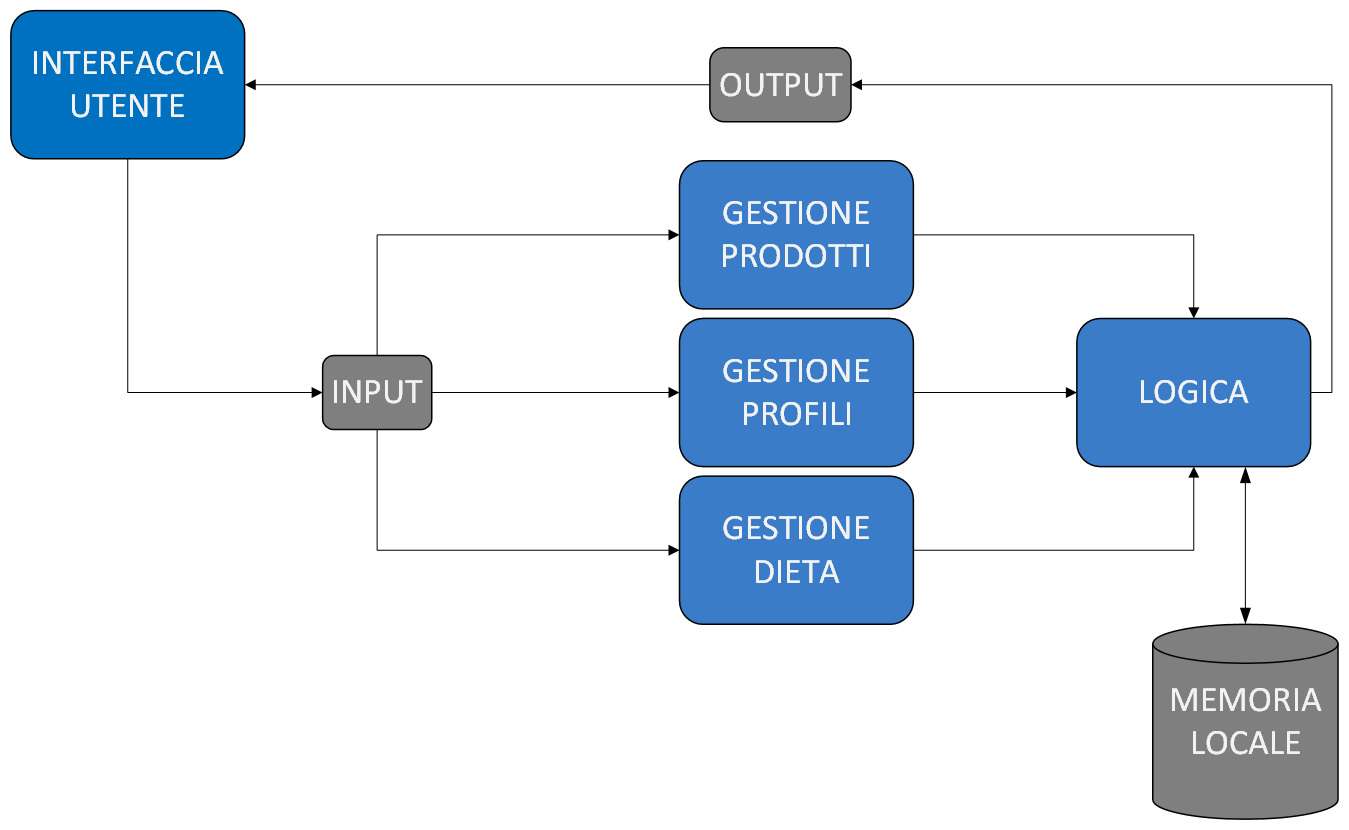
\includegraphics[width=0.8\textwidth]{imgs/VistaModuloUso.png}
    \caption{Punto di vista del modulo con relazione "Usa"}
    \label{fig:enter-label}
\end{figure}
\subsubsection{Punti di vista dei Componenti e dei Connettori (Vista Dinamica)}

\begin{figure}[H]
    \centering
    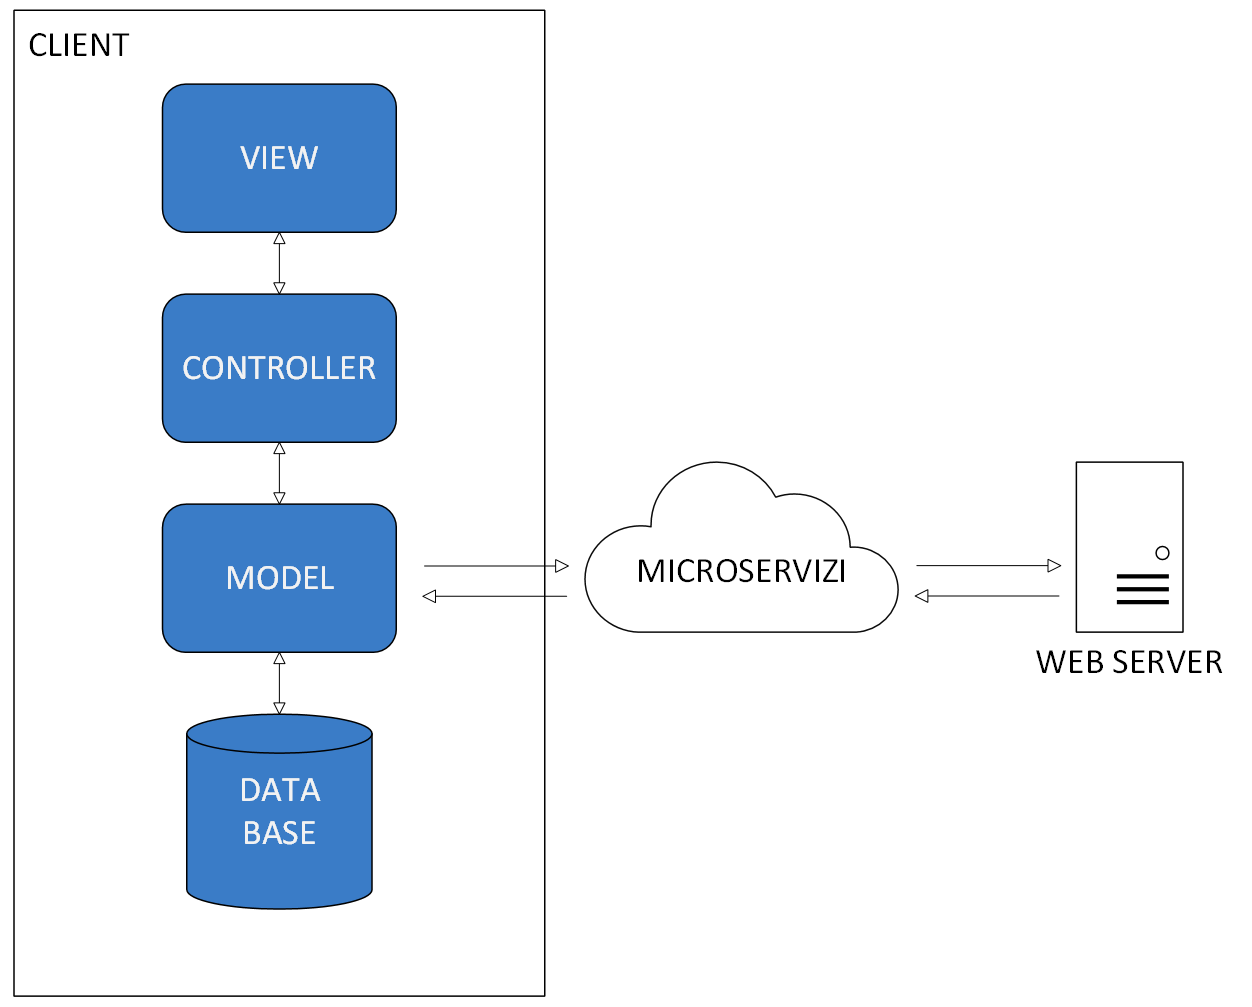
\includegraphics[width=0.8\textwidth]{imgs/Vista.png}
    \caption{Punto di vista dei componenti e dei connettori}
    \label{fig:enter-label}
\end{figure}

La struttura del client è quella che verrà effettivamente sviluppata e utilizzata come riferimento per lo sviluppo del software; i microservizi sono considerati un possibile ampliamento dell'architettura ma che non sarà implementata nella versione finale del software. Inoltre, le relazioni simboleggiate da due frecce distinte in direzione opposta indicano che la relazione è su richiesta, e non un continuo scambio di dati tra i componenti.  
\section{Design}


\end{document}
